\newslide{Altitude Keeping}{
	\begin{columns}[c]
	\column{0.2\textwidth}
	\begin{tikzpicture}[>=latex',scale=0.4]
	\drawplanexy{-0.3}{-0.3}{-0.3}{6.7}{10}{dashed}{perception}
	
	\drawcube{0}{0}{5}{6.4}{1}{white}{dinamica}{}{};
	\drawcube{0}{1.2}{5}{6.4}{1}{white}{tracking}{}{};
	
	\drawcube{0}{2.4}{5}{6.4}{1}{white}{ostacoli}{}{};
	\drawcube{0}{3.6}{5}{6.4}{1}{gray!40}{altitude}{}{};
	
	\drawcube{0}{4.8}{5}{3}{1.5}{white}{source}{}{};
	\drawcube{0}{6.5}{5}{3}{1.5}{white}{emulatore}{}{};

	\drawplanezy{3.2}{4.8}{5}{4.5}{radar_det}{fill=white,opacity=0.90}{}{};

	\drawcube{3.4}{4.8}{5}{3}{3.2}{white}{alpha}{}{};
	\drawplanexy{-0.3}{-0.3}{5.3}{6.7}{10}{dashed}{action}
	

	\draw [->,line width=1.5] (action_D) -- ++(0,0,2);
	\draw [->,line width=1.5] (perception_D) -- ++(0,0,2);

	\coordinate [at=(radar_det_D), yshift=-5] (arrows_point);
	\draw [->,dashed]  (arrows_point) -- ++(1.5,0,0); 
	\draw [->,dashed]  (arrows_point) -- ++(-1.5,0,0); 
	\end{tikzpicture}
	\vspace{6.5cm}
	\column{0.8\textwidth}
	\begin{block}{}
		\centering
		Identification of the surface normal $\mathbf{m}$ $\longrightarrow$ S.L.A.M. Problem $\left[\begin{array}{c} \mathbf{x} \\  \mathbf{m} \end{array}\right]$
		\vspace{0.45cm}
		
		\begin{tikzpicture}
			\node (immagine) {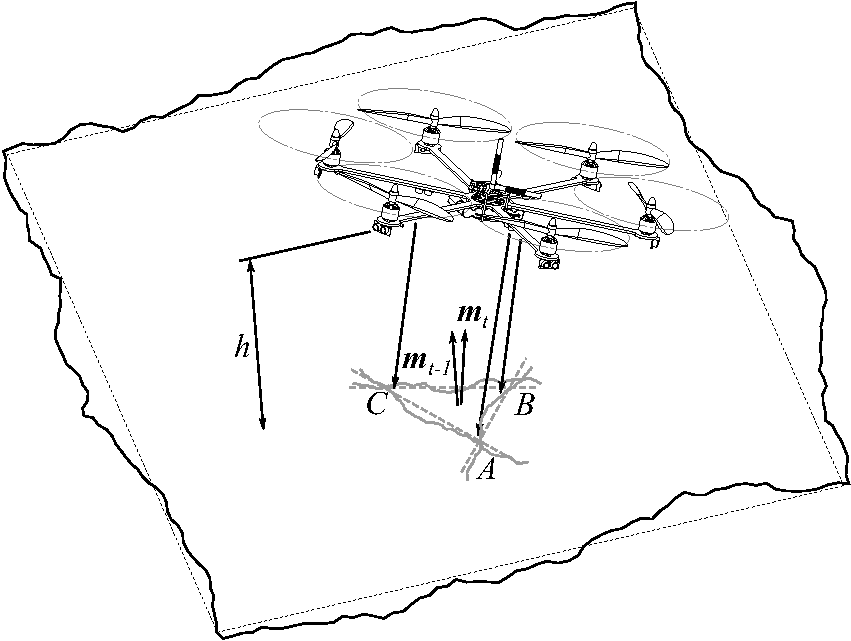
\includegraphics[scale=0.7]{img/altitude_keep.pdf}};
			\node [at=(immagine.south east), anchor=mid,yshift=1cm] {$\mathbf{m}_t=\dfrac{(A-B)\times(B-C)}{|(A-B)\times(B-C)|}$};
		\end{tikzpicture}
		\vspace{0.45cm}

		Keep the VTOL at costant distance $h$ along exstimated plane normal $\mathbf{m}_t$
	\end{block}
	\end{columns}
}